\documentclass [12pt]{article}


\usepackage{ucs}
\usepackage[utf8x]{inputenc} %Поддержка UTF8
\usepackage{cmap} % Улучшенный поиск русских слов в полученном pdf-файле
\usepackage[english,russian]{babel} %Пакет для поддержки русского и английского языка
\usepackage{graphicx} %Поддержка графиков
\usepackage{float} %Поддержка float-графиков
\usepackage[left=20mm,right=15mm, top=20mm,bottom=20mm,bindingoffset=0cm]{geometry}
\usepackage{mathtools} 
\DeclarePairedDelimiter{\abs}{\lvert}{\rvert}
\renewcommand{\baselinestretch}{1.2}
 
\usepackage{color} 
\definecolor{deepblue}{rgb}{0,0,0.5}
\definecolor{deepred}{rgb}{0.6,0,0}
\definecolor{deepgreen}{rgb}{0,0.5,0}
\definecolor{gray}{rgb}{0.5,0.5,0.5}

\DeclareFixedFont{\ttb}{T1}{txtt}{bx}{n}{12} % for bold
\DeclareFixedFont{\ttm}{T1}{txtt}{m}{n}{12}  % for normal

\usepackage{listings}
 
\lstset{
	language=Python,
	basicstyle=\ttm,
	otherkeywords={self},             % Add keywords here
	keywordstyle=\ttb\color{deepblue},
	emph={MyClass,__init__},          % Custom highlighting
	emphstyle=\ttb\color{deepred},    % Custom highlighting style
	stringstyle=\color{deepgreen},
	frame=tb,                         % Any extra options here
	showstringspaces=false            % 
}
 
\usepackage{hyperref}
 
\hypersetup{
    bookmarks=true,         % show bookmarks bar?
    unicode=false,          % non-Latin characters in Acrobat’s bookmarks
    pdftoolbar=true,        % show Acrobat’s toolbar?
    pdfmenubar=true,        % show Acrobat’s menu?
    pdffitwindow=false,     % window fit to page when opened
    pdfstartview={FitH},    % fits the width of the page to the window
    pdftitle={My title},    % title
    pdfauthor={Author},     % author
    pdfsubject={Subject},   % subject of the document
    pdfcreator={Creator},   % creator of the document
    pdfproducer={Producer}, % producer of the document
    pdfkeywords={keyword1} {key2} {key3}, % list of keywords
    pdfnewwindow=true,      % links in new PDF window
    colorlinks=true,       % false: boxed links; true: colored links
    linkcolor=black,          % color of internal links (change box color with linkbordercolor)
    citecolor=green,        % color of links to bibliography
    filecolor=magenta,      % color of file links
    urlcolor=cyan           % color of external links
}

\title{}
\date{}
\author{}

\begin{document}
\begin{titlepage}
\thispagestyle{empty}
\begin{center}
Федеральное государственное бюджетное образовательное учреждение высшего профессионального образования \\Московский государственный технический университет имени Н.Э. Баумана

\end{center}
\vfill
\centerline{\large{Лабораторная работа №4}}
\centerline{\large{по курсу <<Численные методы>>}}
\centerline{\large{<<Решение нелинейных уравнений>>}}
\vfill
\hfill\parbox{5cm} {
           Выполнил:\\
           студент группы ИУ9-62 \hfill \\
           Иванов Георгий\hfill \medskip\\
           Проверила:\\
           Домрачева А.Б.\hfill
       }
\centerline{Москва, 2017}
\clearpage
\end{titlepage}

\textsc{\textbf{Цель:}} 

Сравнительный анализ численных методов для решения нелинейных уравнений вида: $$f(x)=0$$
\begin{enumerate}
\item Метод деления пополам (метод бисекции)
\item Метод золотого сечения
\end{enumerate}

\textsc{\textbf{Постановка задачи:}}

\textbf{Дано:}  Нелинейное уравнение $f(x)=0$, где $f(x)$ - функция, определенная и непрерывная на некотором промежутке. Функция $f(x)$ может быть задана в виде алгебраического многочлена (полинома некоторой степени) или трансцендентной функции.

В нашем случае, в качестве $f(x)$ возьмем алгебраический многочлен третьей степени, общий вид которого следующий: $f(x)=Ax^3+Bx^2+Cx+D$

Уравнение примет вид:  $$Ax^3+Bx^2+Cx+D=0$$

 \textbf{Найти:} Корни нелинейного уравнения, т.е числа $x_1, x_2, ... , x_n$, которые путём подстановки их в данное уравнение превращают уравнение в верное числовое равенство.

\textbf{Тестовый пример:} $$ 3x^3-8x^2-11x+10=0$$ 

 Корни уравнения:
$$x_1 = 1-\sqrt{6}$$ 
$$x_2 = \frac{2}{3}$$
$$x_3 = 1+\sqrt{6}$$

\textsc{\textbf{Теоретические сведения:}}

Решение линейных уравнений - нахождение корней функции $f(x)$. Корнем функции $f(x)$ называют такое значение, при котором $f(x)=0$. При этом визуально задача сводится к нахождению точки пересечения графика функции $f(x)$ с осью абсцисс.

Если уравнение достаточно сложно (в аналитическом плане), то задача точного определения корней является в некоторых случаях нерешаемой. Поэтому ставится задача найти такое приближенное значение корня $x_{пр}$, которое отличается от точного значения корня $x^{*}$ на величину, по модулю не превышающую указанной точности (малой положительной величины)  $\varepsilon$, то есть
$$ \abs{x^{*}  - x_{пр}}< \varepsilon $$

Величину  $\varepsilon$ также называют допустимой ошибкой, которую можно задать по своему усмотрению.

Для нахождения приближенного решения уравнения нам необходимо:
\begin{itemize}
\item Отделить корни, то есть найти интервалы из области определения функции $f(x)$, в каждом из которых содержится только один корень уравнения $f(x)=0$.
\item Уточнить корни до заданной точности
\end{itemize}

Отделение корней можно проводить графически и аналитически.
Для того чтобы графически отделить корни уравнения, необходимо построить график функции $f(x)$. Абсциссы точек его пересечения с осью абсцисс являются корнями уравнения. Но при этом аналитическое отделение корней возможно только лишь на отрезках, принимающих значения разных знаков. Из непрерывности функции $f(x)$,т.е $f(a)*f(b)<0$ следует, что на отрезке $[a;b]$ содержится по крайней мере один корень уравнения.

В нашем случае мы отделим наше уравнение тремя отрезками $[-2;0]$, $[0;2]$, $[2;4]$.
\begin{figure}[h]
\begin{center}
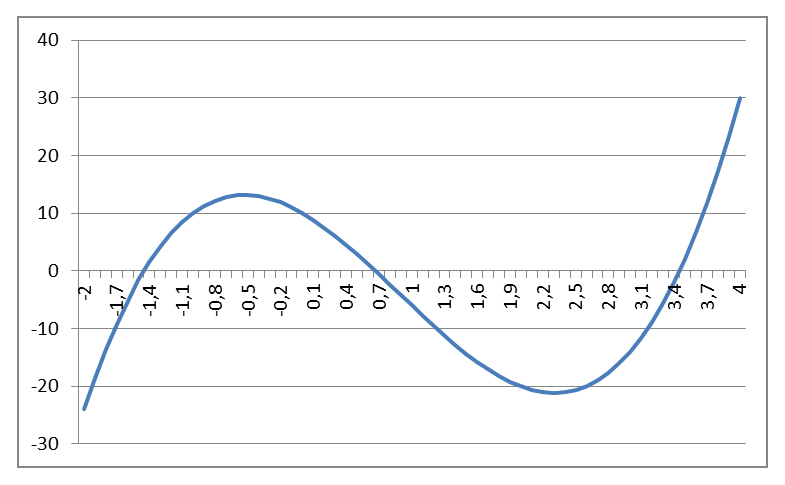
\includegraphics[scale=.9]{1.eps}\\
\textit{Рисунок 1. График функции $y=3x^3-8x^2-11x+10$}
\end{center}
\end{figure}

Для уточнения корней может использоваться один из различных численных методов для решения нелинейных уравнений.  В ходе данной лабораторной работы рассмотрим метод деления пополам (метод бисекции) и метод золотого сечения.

\textbf{1. Метод деления пополам}

Суть метода деления отрезка пополам состоит в:
\begin{itemize}
\item Разбиение отрезка $[a;b]$ (при условии $f(a)*f(b)<0$) на два отрезка
\item Определение знака функции $f(x)$ в точке $x_m=\frac{a+b}{2}$
\item Выбор отрезка, на котором функция меняет знак и содержит решение
\end{itemize}

Отрезок, для которого условие смены знака ($f(a)*f(b)<0$) не выполняется, отбрасываем. 
После каждой итерации отрезок, на котором расположен корень, уменьшается в два раза, а после  $n$ итераций - в $2^n$ раз.
Теперь этот отрезок снова делим пополам и оставляем ту его часть, на границах которой функция имеет разные знаки, и так далее, достижения требуемой точности решения $\varepsilon$. Условие остановки деления отрезка: $$ \abs{b - a}>2\varepsilon $$

После завершения итерационного процесса получаем корень $x_m$

\textbf{2.  Метод золотого сечения}

Данный метод является улучшенным методом наивной реализации троичного поиска

Суть метода золотого сечения состоит в:
\begin{itemize}
\item Деление отрезка $[a;b]$ в пропорции золотого сечения в обоих направлениях $x_1,x_2$
\\ ($x_1=a+\frac{b-a}{\varphi}$,$x_2=b-\frac{b-a}{\varphi}$)
\\ где $\varphi$ - пропорция золотого сечения ($\varphi=\frac{1+\sqrt{5}}{2}$)
\item Определение знака функции $f(x)$ в точках $x_1=a+\frac{b-a}{\varphi}$ и $x_2=b-\frac{b-a}{\varphi}$
\item Выбор отрезка, на котором функция меняет знак и содержит решение. 
\\ Сначала делаем проверку отрезка $[x1;x2]$. 
\\ Если меняет знак ($f(x1)*f(x2)<0$), то переходим к следующей итерации, где исследуемым отрезком будет $[x1;x2]$, иначе  переходим к проверке отрезка $[a;x2]$.
\\ Если меняет знак ($f(a)*f(x2)<0$), то переходим к следующей итерации, где исследуемым отрезком будет $[a;x2]$, иначе исследуемым отрезком будет $[x1;b]$
\end{itemize}

Теперь этот отрезок снова делим в пропорции золотого сечения в обоих направлениях и оставляем ту его часть, на границах которой функция имеет разные знаки, и так далее, достижения требуемой точности решения $\varepsilon$. Условие остановки деления отрезка: $$ \abs{b - a}>2\varepsilon $$

После завершения итерационного процесса получаем корень $x=\frac{a+b}{2}$

\textsc{\textbf{Практическая реализация:}}
Листинг 1. Методы решения нелинейных уравнений
\begin{lstlisting}[language=python]

#!python
# -*- coding: utf-8 -*-

import math

def func(x):
    return 3*x ** 3 - 8*x**2 - 11*x + 10

def bisection_method(func,a,b,eps):
    if func(a)==0:
        return a
    elif func(b)==0:
        return b
    x = (a + b) / 2
    iteration = 0
    while abs(b-a)>2*eps:
        x = (a+b) / 2
        iteration += 1
        if func(a)*func(x)<0:
            b = x
        else:
            a = x
    return (iteration,(a+b)/2)

def golden_method(func,a,b,eps):
    iteration = 0
    phi = (1 + math.sqrt(5)) / 2
    while abs(b-a)>2*eps:
        iteration += 1
        x1 = b - (b - a) / phi
        x2 = a + (b - a) / phi
        if func(x1)*func(x2)<0:
            a = x1
            b = x2
        else:
            if func(a)*func(x2)<0:
                b = x2
            else:
                a = x1
    return (iteration,(a+b)/2)


if __name__ == "__main__":
    epsilon = [10 ** (-i) for i in range(1, 4)]
    real_answers = [1-math.sqrt(6),2/3,1+math.sqrt(6)]
    print("Bisection method: ")
    for eps in epsilon:
        print(" Epsilon = " + str(eps))
        roots = []
        roots.append(bisection_method(func,-2,0,eps))
        roots.append(bisection_method(func,0,2,eps))
        roots.append(bisection_method(func,2,4,eps))
        for i in range(len(roots)):
            print("  Iterations: " + str(roots[i][0]))
            print("  x = " + str(roots[i][1]))
            print("  x_real = " + str(real_answers[i]))
    print("Golden section method: ")
    for eps in epsilon:
        print(" Epsilon = " + str(eps))
        roots = []
        roots.append(golden_method(func, -2, 0, eps))
        roots.append(golden_method(func, 0, 2, eps))
        roots.append(golden_method(func, 2, 4, eps))
        for i in range(len(roots)):
            print("  Iterations: " + str(roots[i][0]))
            print("  x = " + str(roots[i][1]))
            print("  x_real = " + str(real_answers[i]))

\end{lstlisting}

\textsc{\textbf{Результаты:}}

Для тестирования полученной программы было выбрано уравнение, $$ 3x^3-8x^2-11x+10=0$$ имеющее 3 корня:
$$x_1 = 1-\sqrt{6}$$ 
$$x_2 = \frac{2}{3}$$
$$x_3 = 1+\sqrt{6}$$
Так как данные методы находят лишь один корень, поэтому нам пришлось провести отделение корней, в пределах которых корень будет единственный. 
В нашем случае мы отделим наше уравнение тремя отрезками $[-2;0]$, $[0;2]$, $[2;4]$, при этом каждому корню соответствует свой отрезок.
Чтобы количество итераций и вычисляемое значение было корректно, данные отрезки должны быть равны друг другу.


В качестве  $\varepsilon$ для каждого метода были выбраны следующие значения: $$\varepsilon=0.1,\varepsilon=0.01,\varepsilon=0.001$$

Ниже приведена таблица результата полученной программы (Листинг 1) на указанных выше методах:

\begin{center}
\begin{tabular}{ |c|c|c|c|c| }
  \hline
  & \multicolumn{2}{|c|}{Метод бисекций}
  & \multicolumn{2}{|c|}{Метод золотого сечения} \\ \hline
  & Значение & Кол-во итераций & Значение & Кол-во итераций \\ \hline
  & \multicolumn{4}{|c|}{$\varepsilon=0.1$} \\ \hline
  x1 & -1.4375 & 4 & -1.4376941012509463 & 3  \\ \hline
  x2 & 0.6875 & 4 & 0.673762078750736 & 3 \\ \hline
  x3 & 3.4375 & 4 & 3.4376941012509463 & 3 \\ \hline
  & \multicolumn{4}{|c|}{$\varepsilon=0.01$} \\ \hline
  x1 & -1.4453125 & 7 & -1.4508497187473712 & 6  \\ \hline
  x2 & 0.6640625 & 7 & 0.6656314599949527 & 6 \\ \hline
  x3 & 3.4453125 & 7 & 3.450849718747371 & 6 \\ \hline
  & \multicolumn{4}{|c|}{$\varepsilon=0.001$} \\ \hline
  x1 & -1.4501953125 & 10 & -1.449663477457729 & 9  \\ \hline
  x2 & 0.6669921875 & 10 & 0.6668177012845948 & 8 \\ \hline
  x3 & 3.4501953125 & 10 & 3.4496634774577286 & 9 \\ \hline
\end{tabular}
\end{center}

\textsc{\textbf{Выводы:}}

В ходе выполнения лабораторной работы были рассмотрены два численных метода решения нелинейных уравнений вида: $f(x)=0$: метод деления пополам (метод бисекции), метод золотого сечения. Была написана реализация данных методов на языке программирования Python.

Сравнивая результаты в таблице вычислений, метод золотого сечения является более точным по сравнению с методом бисекций (меньшее количество итераций и более точный результат вычислений). Хоть и метод бисекций является более простым (в плане реализации) и имеет высокую надежность, метод золотого сечения уменьшает отрезок на каждой итерации алгоритма на величину большую в отличие от метода деления пополам. Стоит заметить, что при больших значениях точности $\varepsilon=0.01$ метод бисекций оказался более точным, но хотя при меньшем значении точности $\varepsilon=0.001$ более точным оказался метод золотого сечения. Это возникает в следствие того, что способ нахождения анализируемого отрезка  при каждой итерации различный в данных методах.

Следовательно, нельзя назвать точно лучший метод для решения нелинейных уравнений.

\end{document}
